\documentclass[10pt,english, openany]{book}

%%%%%%%%%%%%%%%%%%%%%%%%%%%%%% Loading packages that alter the style
\usepackage[]{graphicx}
\usepackage[]{color}
\usepackage{alltt}
\usepackage[T1]{fontenc}
\usepackage[utf8]{inputenc}
\setcounter{secnumdepth}{3}
\setcounter{tocdepth}{3}
\setlength{\parskip}{\smallskipamount}
\setlength{\parindent}{0pt}

% Set page margins
\usepackage[top=100pt,bottom=100pt,left=68pt,right=66pt]{geometry}

% Package used for placeholder text
\usepackage{lipsum}

% Prevents LaTeX from filling out a page to the bottom
\raggedbottom

% Adding both languages
\usepackage[english, italian]{babel}

% All page numbers positioned at the bottom of the page
\usepackage{fancyhdr}
\fancyhf{} % clear all header and footers
\fancyfoot[C]{\thepage}
\renewcommand{\headrulewidth}{0pt} % remove the header rule
\pagestyle{fancy}

% Changes the style of chapter headings
\usepackage{titlesec}
\titleformat{\chapter}
   {\normalfont\LARGE\bfseries}{\thechapter.}{1em}{}
% Change distance between chapter header and text
\titlespacing{\chapter}{0pt}{50pt}{2\baselineskip}

% Adds table captions above the table per default
\usepackage{float}
\floatstyle{plaintop}
\restylefloat{table}

% Adds space between caption and table
\usepackage[tableposition=top]{caption}

% Adds hyperlinks to references and ToC
\usepackage{hyperref}
\hypersetup{hidelinks,linkcolor = black} % Changes the link color to black and hides the hideous red border that usually is created

% If multiple images are to be added, a folder (path) with all the images can be added here 
\graphicspath{ {Figures/} }

% Separates the first part of the report/thesis in Roman numerals
\frontmatter
\usepackage{listings}

%%%%%%%%%%%%%%%%%%%%%%%%%%%%%% Starts the document
\begin{document}

%%% Selects the language to be used for the first couple of pages
\selectlanguage{english}

%%%%% Adds the title page
\begin{titlepage}
	\clearpage\thispagestyle{empty}
	\centering
	\vspace{0.5cm}    
    \centering 
\includegraphics[scale=0.5]{agh.jpg}    
	\vspace{0.5cm}   
	
		\vspace{2cm}
	{\huge \textbf{Metody programowania równoległego}} \\
	\vspace{0.5cm} 
	{\Huge \textbf{Sprawozdanie z mierzenia opóźnienia i przepustowości w klastrze}} \\
	\vspace{6cm}	
	{\Large autor: Ilona Tomkowicz\\}
	\vspace{0.5cm} 
	{\Large Akademia Górniczo-Hutnicza\\
	Wydział Informatyki, Elektroniki i Telekomunikacji,\\
	Informatyka, II stopień, I semestr \par}
	   \vspace{0.5cm} 
	% Set the date
	{\Large 08 marca 2020 \par}
	
	\pagebreak

\end{titlepage}

% Adds a table of contents
\tableofcontents{}

%%%%%%%%%%%%%%%%%%%%%%%%%%%%%%%%%%%%%%%%%%%%%%%%%%%%%%%%%%%%%%%%%%%%%%%%%%%%%%%%%%%%%%%%%%%%
%%%%%%%%%%%%%%%%%%%%%%%%%%%%%%%%%%%%%%%%%%%%%%%%%%%%%%%%%%%%%%%%%%%%%%%%%%%%%%%%%%%%%%%%%%%%
%%%%% Text body starts here!
\mainmatter
%1. kodów programów
%2. danych pomiarowych
%3. pomiarów opóźnienia i wykresów przepustowości dla różnych parametrów / konfiguracji - może być w osobnych plikach lub złożone w formie dokumentu, np. PDF. Wykresy mają mieć opisane osie oraz informacje o konfiguracji w jakiej test został uruchomiony (jakie maszynki, jakie parametry etc).
%4. wniosków do wykresów

\chapter{Kody źródłowe}\label{chapt:kod}
\section{Komunikacja z użyciem Send i Recv}
\lstinputlisting[language=C]{codes/hw.c}

\section{Komunikacja z użyciem Isend i Irecv}
\lstinputlisting[language=C]{codes/hw_b.c}

\section{Komunikacja z użyciem jednego węzła i pamięci współdzielonej}
Konfiguracja pliku allnodes zawierała tylko adres tego węzła, a program uruchamiano na tym samym węźle.
\lstinputlisting[language=C]{codes/hosts}

\section{Komunikacja z użyciem jednego węzła i połączenia sieciowego}
Konfiguracja pliku allnodes zawierała tylko adres tego węzła, a program uruchamiano na innym węźle, w tym wypadku na 02.

\section{Komunikacja z użyciem dwóch węzłów, będących fizycznie na tej samej maszynie i połączenia sieciowego}
Konfiguracja pliku allnodes zawierała adresy używanych węzłów (01, 03), a program uruchamiano na węźle 02.
\lstinputlisting[language=C]{codes/hosts_2}

\section{Komunikacja z użyciem dwóch węzłów, będących fizycznie na różnych maszynach i połączenia sieciowego}
Konfiguracja pliku allnodes zawierała adresy używanych węzłów (05, 06), a program uruchamiano na węźle 02.
\lstinputlisting[language=C]{codes/hosts_3}

\chapter{Dane pomiarowe}

Pomiary wykonano dla paczek od 64 B do 

\begin{table}[H]
\caption{Jeden węzeł, pamięć współdzielona}
\begin{center}
\begin{tabular}{|c|c|}
\hline
rozmiar {[}bit{]} & Send/recv przepustowość {[}Mbit/s{]} \\ \hline
64              & 347.872                              \\ \hline
256             & 1328.89                              \\ \hline
1024            & 4148.32                              \\ \hline
4096            & 12235.5                              \\ \hline
16384           & 38741.4                              \\ \hline
65536           & 60750.5                              \\ \hline
262144          & 61720.4                              \\ \hline
1048576         & 51421.7                              \\ \hline
\end{tabular}
\end{center}
\end{table}

\begin{table}[H]
\caption{Jeden węzeł, pamięć współdzielona}
\begin{center}
\begin{tabular}{|c|c|}
\hline
size {[}bit{]} & Isend/Irecv przepustowość {[}Mbit/s{]} \\ \hline
64           & 75.871                                 \\ \hline
256          & 322.474                                \\ \hline
1024         & 1240.93                                \\ \hline
4096         & 7566.22                                \\ \hline
16384        & 27147.9                                \\ \hline
65536        & 81429.6                                \\ \hline
262144       & 119653                                 \\ \hline
1048576      & 55264.7                                \\ \hline
\end{tabular}
\end{center}
\end{table}


\begin{table}[H]
\caption{Jeden węzeł, połączenie sieciowe}
\begin{center}
\begin{tabular}{|c|c|}
\hline
size {[}bit{]} & Send/recv przepustowość {[}Mbit/s{]} \\ \hline
64           & 339.148                              \\ \hline
256          & 1354.45                              \\ \hline
1024         & 4119.87                              \\ \hline
4096         & 13120.9                              \\ \hline
16384        & 36961.9                              \\ \hline
65536        & 46702.7                              \\ \hline
262144       & 54996.8                              \\ \hline
\end{tabular}
\end{center}
\end{table}

\begin{table}[H]
\caption{Jeden węzeł, połączenie sieciowe}
\begin{center}
\begin{tabular}{|c|c|}
\hline
size {[}bit{]} & Isend/Irecv przepustowość {[}Mbit/s{]} \\ \hline
64           & 74.3444                                \\ \hline
256          & 275.714                                \\ \hline
1024         & 1601.85                                \\ \hline
4096         & 4002.86                                \\ \hline
16384        & 25237.1                                \\ \hline
65536        & 71933.1                                \\ \hline
262144       & 75605.2                                \\ \hline
1048576      & 43859.2                                \\ \hline
\end{tabular}
\end{center}
\end{table}

\begin{table}[H]
\caption{Dwa węzły, jeden host}
\begin{center}
\begin{tabular}{|c|c|}
\hline
size {[}bit{]} & Send/recv przepustowość {[}Mbit/s{]} \\ \hline
64           & 319.243                              \\ \hline
256          & 1156.55                              \\ \hline
1024         & 4638.69                              \\ \hline
4096         & 12530.4                              \\ \hline
16384        & 31242.5                              \\ \hline
65536        & 59722.3                              \\ \hline
262144       & 53988.5                              \\ \hline
\end{tabular}
\end{center}
\end{table}


\begin{table}[H]
\caption{Dwa węzły, jeden host}
\begin{center}
\begin{tabular}{|c|c|}
\hline
size {[}bit{]} & Isend/Irecv przepustowość {[}Mbit/s{]} \\ \hline
64           & 74.64                                  \\ \hline
256          & 337.766                                \\ \hline
1024         & 1003.36                                \\ \hline
4096         & 4407.19                                \\ \hline
16384        & 26874.5                                \\ \hline
65536        & 60076.7                                \\ \hline
262144       & 120085                                 \\ \hline
1048576      & 36403.5                                \\ \hline
\end{tabular}
\end{center}
\end{table}

\begin{table}[H]
\caption{Dwa węzły, różne hosty}
\begin{center}
\begin{tabular}{|c|c|}
\hline
size {[}bit{]} & Send/recv przepustowość {[}Mbit/s{]} \\ \hline
64           & 3.09821                              \\ \hline
256          & 12.1787                              \\ \hline
1024         & 49.11                                \\ \hline
4096         & 76.0858                              \\ \hline
16384        & 120.212                              \\ \hline
65536        & 440.153                              \\ \hline
262144       & 1206.13                              \\ \hline
524288       & 1917.71                              \\ \hline
\end{tabular}
\end{center}
\end{table}

\begin{table}[H]
\caption{Dwa węzły, różne hosty}
\begin{center}
\begin{tabular}{|c|c|}
\hline
size {[}bit{]} & Isend/Irecv przepustowość {[}Mbit/s{]} \\ \hline
64           & 9.89011                                \\ \hline
256          & 36.2111                                \\ \hline
1024         & 92.1024                                \\ \hline
4096         & 360.693                                \\ \hline
16384        & 895.855                                \\ \hline
65536        & 2388.71                                \\ \hline
262144       & 2862.97                                \\ \hline
1048576      & 3153.6                                 \\ \hline
\end{tabular}
\end{center}
\end{table}

\begin{table}[H]
\caption{Porównanie opóźnienia dla małej paczki 64 bitów}
\begin{center}
\begin{tabular}{|c|c|l|}
\hline
       & Send+Recv       & Isend+Irecv     \\ \hline
zad\_1 & 1.94335e-07 sec & 7.73275e-07 sec \\ \hline
zad\_2 & 2.21586e-07 sec & 8.59272e-07 sec \\ \hline
zad\_3 & 1.99199e-07 sec & 8.57234e-07 sec \\ \hline
zad\_4 & 2.06115e-05 sec & 6.07103e-06 sec \\ \hline
\end{tabular}
\end{center}
\end{table}

\chapter{Wykresy dla różnych konfiguracji}

\centering 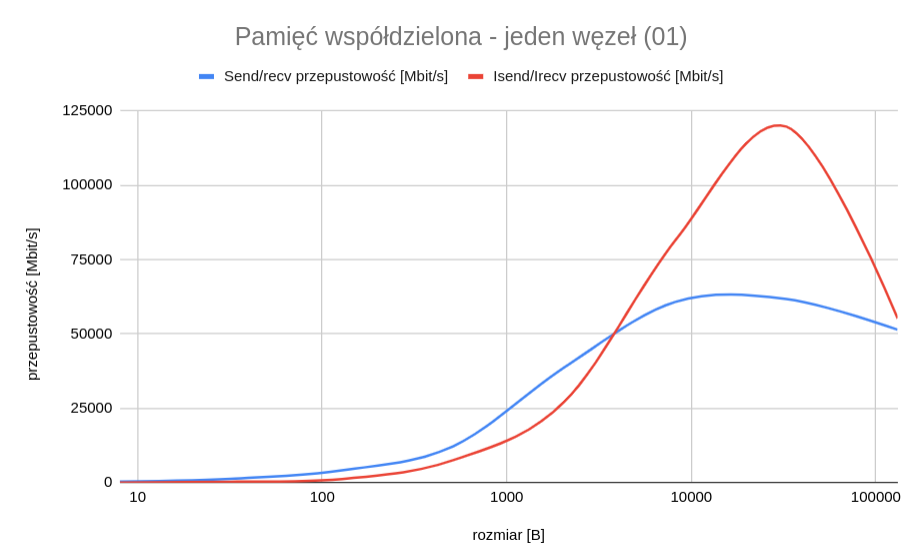
\includegraphics[scale=0.65]{pics/z1.png}    
\centering 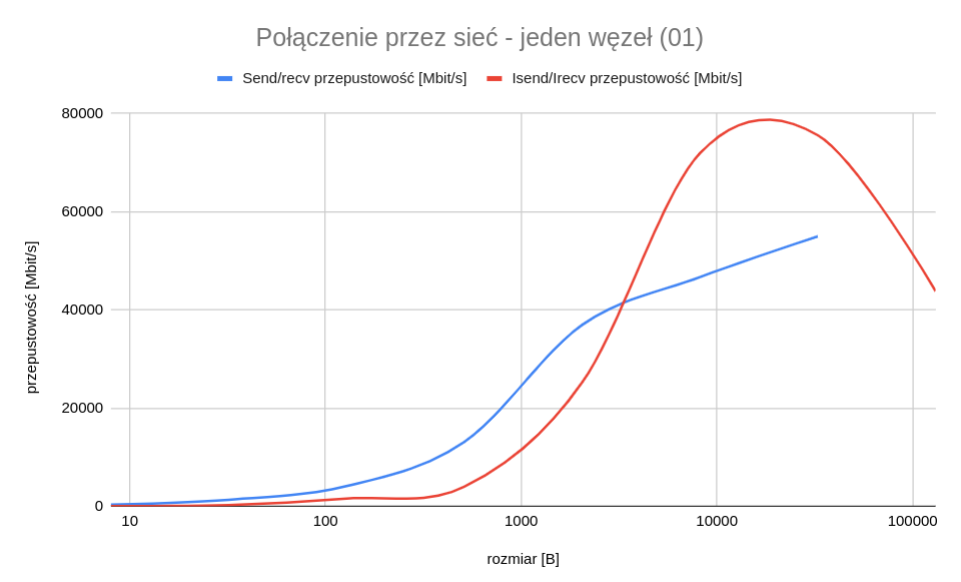
\includegraphics[scale=0.63]{pics/z2.png}    
\centering 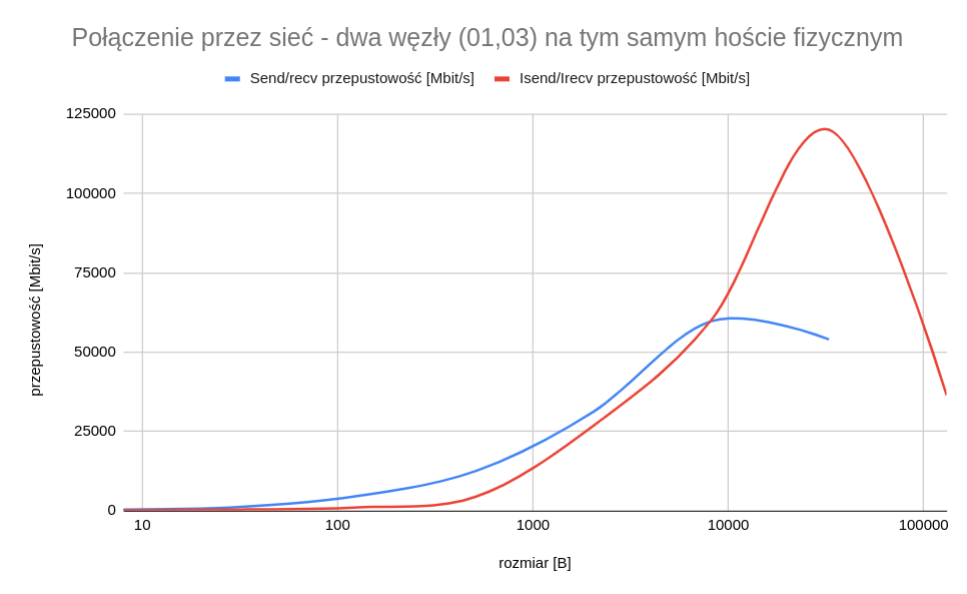
\includegraphics[scale=0.63]{pics/z3.png}    
\centering 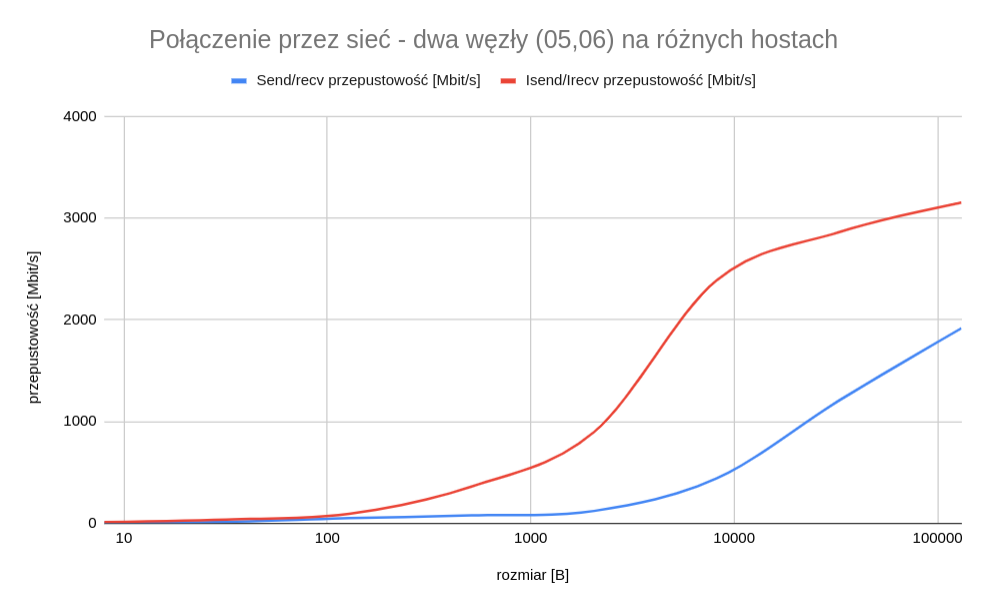
\includegraphics[scale=0.6]{pics/z4.png}    

\chapter{Wnioski}

\end{document}